\chapter{Compensatory Mutations}
\label{cm:chapter}
As motivated in the introduction, we introduce \emph{compensatory mutations}
into the classical model of Muller's ratchet in this chapter. Therefore we
assume that every acquired mutation has a probability $\gamma \in [0,1]$ to
become compensated.
At first, we take a brief look at an extended version of Haigh's discrete model. As results are
difficult to derive here, we will soon go on to two time-continuous approximations that have proved
to be useful for the classical model. The first one is the popular diffusion approximation of
Muller's ratchet, a Fleming-Viot process described in \cite{etheridge_how_2008}.
Similar to the approximation for the discrete model, the second one is the (weak) large population
limit of the diffusion approximation, which is almost surely deterministic. This model is
defined as the solution of an ordinary differential equation (ODE), while the
diffusion limit relies on a stochastic differential equation (SDE). Hence, we refer to the latter model as ODE approximation
of Muller's ratchet. We will introduce both models directly including compensatory mutations.
However, we do explicitly allow $\gamma = 0$, i.e. the absence of such mutations. In this case, in
particular the results about the ODE approximation are well-known (see \cite{etheridge_how_2008}).

Our agenda for this chapter is similar to the  previous one. First we
show that the SDE has a unique solution (Theorem~\ref{da:t:eau}, p.~\pageref{da:t:eau}). For that, it will be crucial to
reformulate the SDE as a martingale problem (Theorem~\ref{da:t:SDE=MP}, p.~\pageref{da:t:SDE=MP}).
Afterwards, we show that the ODE approximation is indeed a (weak) limit of solutions of the SDE
(Theorem~\ref{ode:t:SDE->ODE}, p.~\pageref{ode:t:SDE->ODE}) and that the ODE is well-posed
(Theorem~\ref{ode:t:ode_uniqueness}, p.~\pageref{ode:t:ode_uniqueness}). Then, we will introduce
cumulants and derive the existence of an equilibrium point
(Corollary~\ref{ode:c:ex_stat_point}, p.~\pageref{ode:c:ex_stat_point}). Analogous to the Maia-Botelho-Fontanari-Theorem we
explicitly solve the ODE (Theorem~\ref{ode:t:expl_solution}, p.~\pageref{ode:t:expl_solution}) using
a stochastic particle system afterwards. Finally we prove that the ODE approximation always
convergences towards the equilibrium point (Corollary~\ref{ode:c:conv_to_theta},
p.~\pageref{ode:c:conv_to_theta}).\footnote{The results in this chapter are
joint work of Peter Pfaffelhuber, Anton Wakolbinger and the author. A
shorter version of this manuscript, which is prepared for publication
(\citet{pfaffelhuber_mullers_2011}), is attached in the Appendix. Note that we were
able to relax the conditions on the exponential moments of the ratchet there.}


\section{The Discrete Model}
It is not difficult to introduce compensatory mutations into Haigh's model of Muller's ratchet. For
instance, we can add an additional step between steps (i) and (ii) in
Definition~\ref{mr:def:mr} by removing a $\Bin{H_i}{\gamma}$-distributed number
$K_i$ of mutations from every individual. Hence the conditioned expectation $p_k$ in \eqref{mr:eq:p_k} changes to
\begin{equation*} \label{cm:eq:p_k-def}
\begin{aligned}
p_k(t+1) &:= \CPR{H_1+J_1-K_1=k}{\mrT{t}} \\
&= \sum_{i=0}^k \PR{J_1=k-i} 
	\sum_{j=i}^\infty \CPR{H_1 = j}{\mrT{t}} \cdot \CPR{K_1 =j-i}{\mrT{t},H_1 = j} \\ 
&= \sum_{i=0}^k e^{-\lambda} \frac{\lambda^{(k-i)}}{(k-i)!}
	\sum_{j=i}^\infty \frac{(1-s)^{j} \cdot \mrKT{j}{t}}{W(t)} 
					  \binom{j}{j-i} \gamma^{j-i} (1-\gamma)^{i}.
\end{aligned}
\end{equation*}

\noindent
With compensatory mutations present, an individual can have less mutations than its parent.
Hence, clicks can be reverted and the ratchet mechanism breaks
(Figure~\ref{cm:f:samplepaths}). In fact, as the expected number of compensatory mutations of an individual with a parent of type
$H_i$ is $\gamma \cdot H_i$, the compensatory effect will increase with an increasing mutational
load of the population. Because the intensity of deleterious mutations is constant, it is reasonable
to assume that the accumulation of mutations slows down and will eventually stop.

\begin{figure}[h]
\begin{center}
	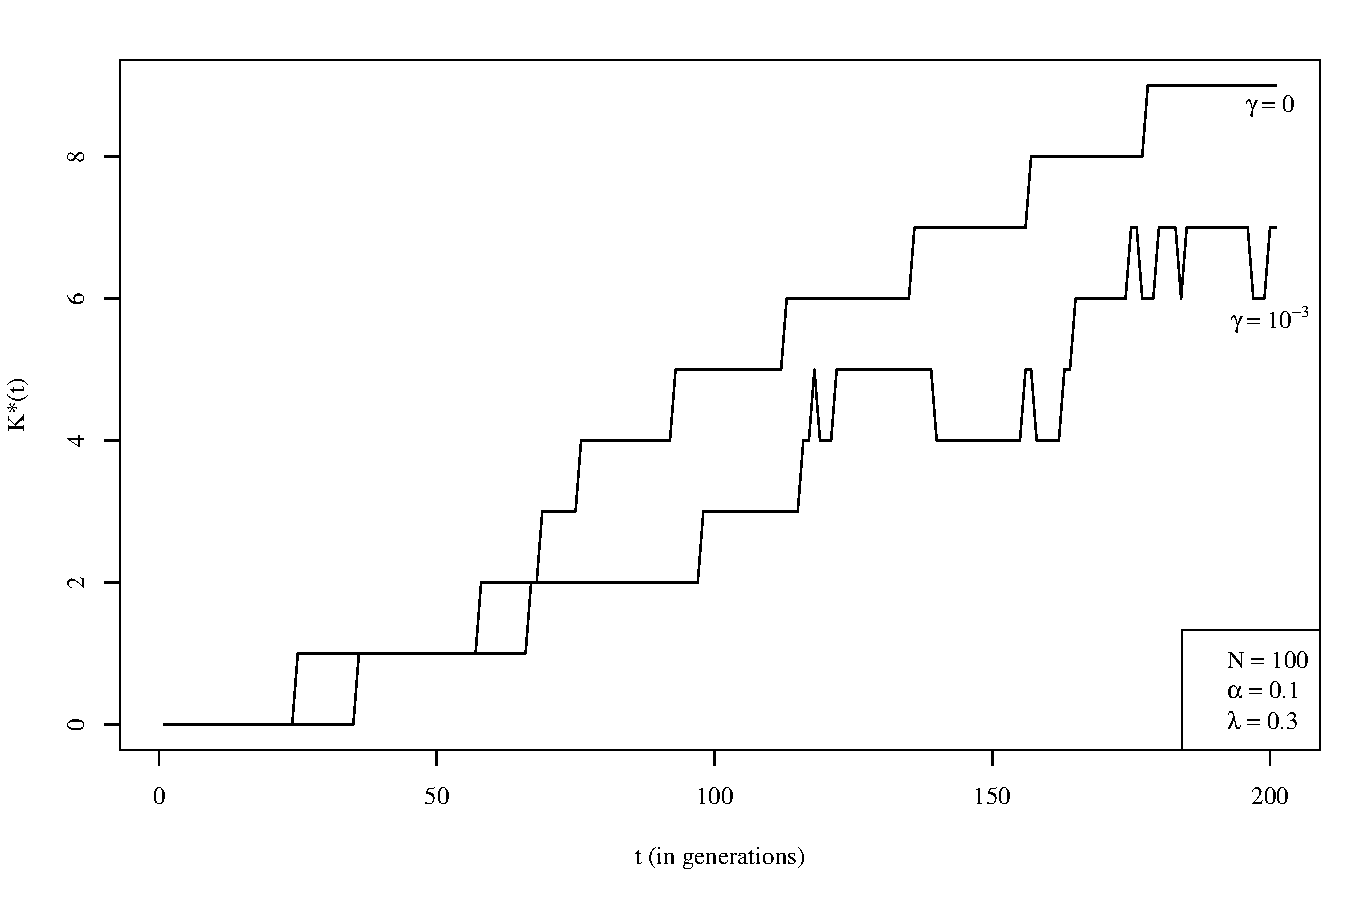
\includegraphics[width=12cm]{img/KSamplePaths}
\end{center}
\caption{\label{cm:f:samplepaths} Evolution of the number of mutations $K^*$ of the fittest class
in time, once non-decreasing without compensatory mutations ($\gamma = 0$) and once also
decreasing with compensatory mutations present ($\gamma = 10^{-3}$).}
\end{figure}

\noindent
Without the ratchet effect present, we can always reach every state in $\Simplex_N$ (as defined in 
\eqref{mr:eq:S_N}) with positive probability. Hence, the ratchet with
compensatory mutations is more similar to the vector of type frequencies
relative to the current fittest class $\Vector{Y}$ in the previous chapter than
to the classical ratchet. Furthermore we can hope that if there is an
equilibrium point, then it is unique. However, the more complicated situation prevents us
from applying any of the approaches we used in the previous chapter. In
particular, we were not able to derive a result similar to the
Maia-Botelho-Fontanari-Theorem for $\gamma > 0$ in the discrete system.
Therefore, we go on to the before mentioned continuous models.